\documentclass[xetex,aspectratio=43]{beamer}

\usepackage{res/lections}

\preamble

\title[Тактовая частота и разрядность]{Тактовая частота и разрядность}

\begin{document}

\titleslide

\tocslide

\section{Характеристики ЭВМ в целом}

\begin{frame}{Характеристики ЭВМ в целом}
    \begin{itemize}
        \item Характеристики процессора
        \item Объём оперативной памяти
        \item Объём и скорость устройств хранения данных
        \item Состав и характеристики интерфейсных устройств
    \end{itemize}
\end{frame}

\begin{frame}{Характеристики процессора}
    \begin{itemize}
        \item Качественная: система команд и архитектура в целом --- об этом позже
        \item Количественная: тактовая частота
        \item Количественная и качественная: разрядность
    \end{itemize}
\end{frame}

\section{Тактовый сигнал}

\begin{frame}{Тактовый сигнал}
    \begin{itemize}
            \item \defn{Тактовый сигнал}{периодический электрический сигнал,
            служащий для синхронизации электронных схем}
            \item \defn{Такт}{промежуток времени между тактовыми
            сигналами}
            \item \defn{Тактовая частота}{частота тактовых сигналов (1/длину такта)}
            \item \defn{Тактовый генератор}{электронная схема, генерирующая тактовый сигнал}
    \end{itemize}

\end{frame}

\begin{frame}[fragile]{Зачем нужен тактовый сигнал? (1)}
    \begin{itemize}
        \tightlist
        \item
        Для многих электронных компонент (например, сумматоров) задано
        максимальное время на операцию
        \item
        Время задаётся в тактах, например

        \begin{itemize}
            \tightlist
            \item
            Для Zilog Z80:

            \begin{itemize}
                \tightlist
                \item
                \mintinline{as}{push RR} (положить значение 16-битного регистра на стек)
                --- 11 тактов
                \item
                \mintinline{as}{pop RR} (снять со стека и сохранить в 16-битном регистре)
                --- 10 тактов
                \item
                \mintinline{as}{add a,R} (прибавить 8-битное значение в регистре
                \mintinline{as}{R} к \mintinline{as}{a}) --- 4 такта
            \end{itemize}
            \item
            Для Intel 80386

            \begin{itemize}
                \tightlist
                \item
                \mintinline{as}{add eax, DWORD PTR [ebp-0x8]} (прибавить к
                32-битному \mintinline{as}{eax} значение из памяти по адресу
                \mintinline{as}{ebp-8}) --- 7 тактов
            \end{itemize}
        \end{itemize}
        \item
        Можно быть уверенным в том, когда операция завершена, а не проверять
        прогресс
    \end{itemize}

    \pause

    \begin{itemize}
        \tightlist
        \item
        На самом деле даже для Intel i80386 это не всегда так, а для более
        новых и подавно
    \end{itemize}
\end{frame}

\begin{frame}{Зачем нужен тактовый сигнал? (2)}
    \begin{itemize}
        \tightlist
        \item
        Ясно, в какой момент можно начинать выполнять следующую команду
        \item
        Ясно, как синхронизировать разные стадии выполнения одной и той же
        команды
        \item
        Ясно, как синхронизировать различные узлы ЭВМ
    \end{itemize}

    При этом

    \begin{itemize}
        \tightlist
        \item
        В ЭВМ обычно много тактовых генераторов и тактовых частот ---
        несколько для ЦП, для ОЗУ (пониже), для шин --- чем дальше
        от ядра процессора, тем ниже
        \item
        Тактовый сигнал не привязан к реальному времени: частота высокая, но
        может «плавать» или понижаться для экономии энергии
    \end{itemize}
\end{frame}

\begin{frame}{Примеры значений тактовой частоты}
        \defn{1 Гц}{(с\({}^{-1}\)), единица частоты периодических событий,
        1 событие в секунду}

        У ЭВМ первого поколения типичное значение тактовой частоты было в
        пределах 100 КГц

        \begin{center}
            \begin{tabular}[]{lrr}
                \hline
                Процессор & Год выпуска & Тактовая частота \\
                \hline
                Intel 4004 & 1971 & 740 КГц \\
                Motorola 6800 & 1974 & 2 МГц \\
                Zilog Z80 & 1976 & 2,5 МГц \\
                Intel 80186 & 1982 & 6 МГц \\
                Intel 80486 DX & 1989 & 20 МГц \\
                Intel 80486 DX4 & 1994 & 100 МГц \\
                Pentium 4 & 2000 & 1,6 ГГц \\
                Intel Xeon Westmere & 2010 & 3,6 ГГц \\
                \hline
            \end{tabular}
        \end{center}

        \pause

        По идее, чем выше, тем «лучше», но у современного сложного процессора
        сигнал за 1 такт не успевает пройти даже от одной части кристалла к другой. Одно из
        косвенных решений --- конвейеризация --- позже
\end{frame}

\begin{frame}{Альтернатива}
    Асинхронные ЭВМ

    \begin{itemize}
        \tightlist
        \item
        Блок процессора / узел внутри ЭВМ подаёт сигнал по мере готовности
        результата
        \item
        Позволяют добиться большей производительности, но сложнее в
        проектировании и устройстве
    \end{itemize}

    Примеры (не экзотические)!

    \begin{itemize}
        \tightlist
        \item
        ILLIAC I и II, GA144 (стековый, дла Forth)
        \item
        Длинные асинхронные операции на современных процессорах, например,
        деление на RISC-процессорах
    \end{itemize}

    \pause

    \begin{itemize}
        \item
        Устройства расширения в «обычных» ЭВМ --- выполняют длительные
        операции (например, с участием DMA), сообщают о выполнении команд и
        получают следующие по мере готовности
    \end{itemize}
\end{frame}

\section{Разрядность}

\begin{frame}{Понятие разрядности}

\begin{itemize}
    \item
    \defn{Разрядность}{обычно --- количество битов в шине данных и в
    машинном слове}
    \item
    \defn{Машинное слово}{минимальная единица обмена данными между
    процессором и ОЗУ}
\end{itemize}

\pause

\begin{block}{А ещё обычно}
    \begin{itemize}
        \tightlist
        \item
        Количество битов в шине данных
        \item
        Количество битов в арифметических регистрах
        \item
        Размер целого числа, над которым аппаратно производится операция
        (машинное слово)
    \end{itemize}
\end{block}

\pause

\begin{block}{И иногда}
    \begin{itemize}
        \tightlist
        \item
        Количество битов в шине адреса и в адресных регистрах
        \item размер стандартного типа
        \mintinline{c}{int} в C (совсем не всегда, может зависеть от архитектуры, ОС и транслятора)
    \end{itemize}
\end{block}

\end{frame}

\begin{frame}{Внутренняя и внешняя разрядность}
\begin{itemize}
    \item
    \defn{Внутренняя разрядность}{количество битов, из которых состоят
    регистры и шины между блоками процессора}
    \item
    \defn{Внешняя разрядность}{количество битов, из которых состоят
    шины компьютера}
\end{itemize}

Обычно речь идёт об арифметических регистрах и шине данных, но понятия внутренней и внешней разрядности также применяются и к адресным регистрам и шине адреса

\end{frame}

\begin{frame}{Примеры, подтверждения и исключения (1): Intel 8086}
\begin{itemize}
    \item
    Шина данных --- 16 битов
    \item
    Арифметические регистры и операции --- по 16 битов

    \begin{itemize}
        \item
        Но \mintinline{as}{mul ax, R/M} считает 32-битный результат
        \mintinline{as}{DX:AX} $\gets$ \mintinline{as}{AX * R/M}
    \end{itemize}
    \item
    Адресные регистры --- 16 битов (адресуют по 64 КиБ)
    \item
    Шина адреса --- 20 битов (16-битный адрес складывается с адресом
    сегмента, это позволяет адресовать до 1 МиБ, об этом позже)

    \pause
    \item
    Intel 8088 (сделан позже 8086, первый процессор IBM PC)

    \begin{itemize}
        \tightlist
        \item
        Всё то же самое, но шина данных 8 битов
    \end{itemize}
\end{itemize}

\end{frame}

\begin{frame}{Примеры, подтверждения и исключения (2): Zilog Z80}
\begin{itemize}
    \item
    Шина адреса --- 16 битов
    \item
    Шина данных --- 8 битов
    \item
    Арифметические регистры и операции --- по 8 битов

    \begin{itemize}
        \item
        Но \mintinline{as}{add hl, bc} считает 16-битный результат над парами
        регистров
    \end{itemize}
\end{itemize}
\end{frame}


\begin{frame}{Примеры, подтверждения и исключения (3)}

\begin{columns}
    \begin{column}{0.5\textwidth}
        \begin{figure}
            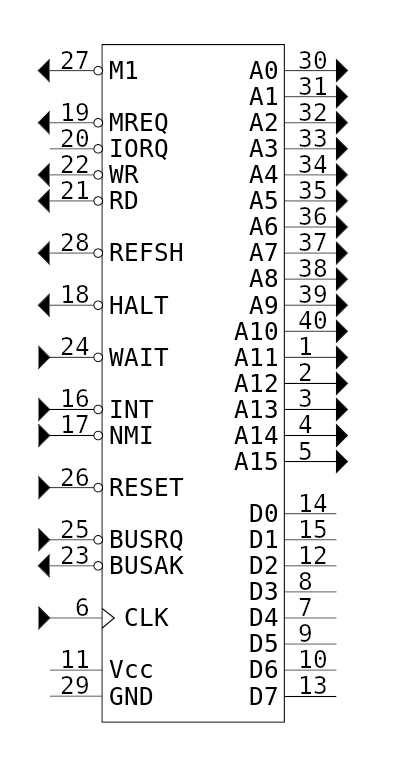
\includegraphics[height=0.8\textheight]{img/05.Zilog_Z80_pinout.png}
            \caption{<<Распиновка>> \href{https://en.wikipedia.org/wiki/Zilog_Z80}{Zilog Z80}}
        \end{figure}
    \end{column}
    \begin{column}{0.5\textwidth}
        \begin{figure}
            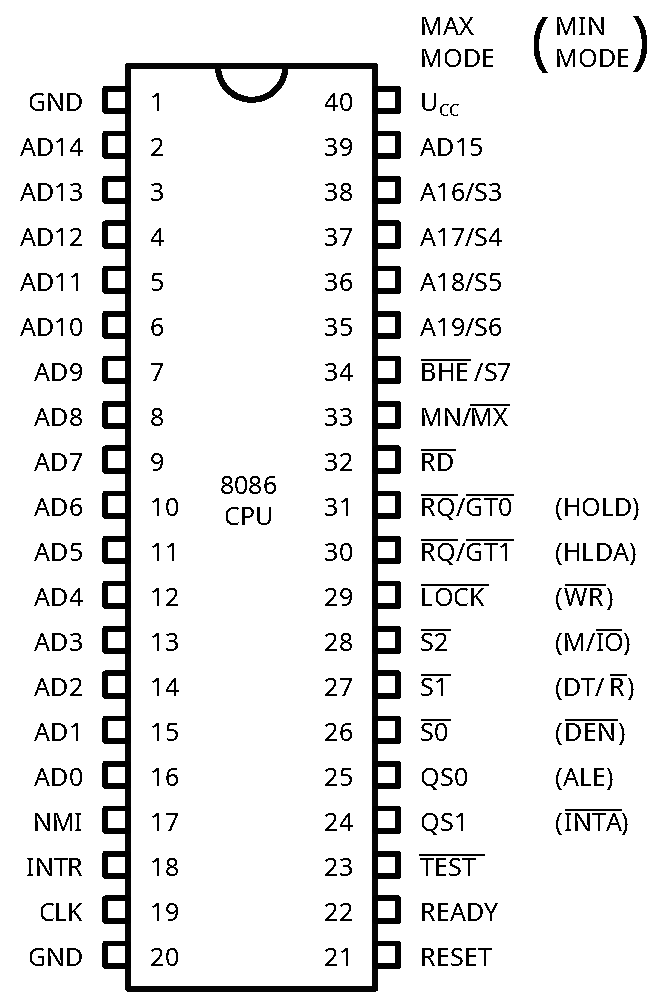
\includegraphics[height=0.75\textheight]{img/05.Intel_8086_pinout.pdf}
            \caption{<<Распиновка>> \href{https://en.wikipedia.org/wiki/Intel_8086}{Intel 8086}}
        \end{figure}
    \end{column}
\end{columns}

\end{frame}

\subsection{Разрядность ОЗУ}

\begin{frame}{Разрядность ОЗУ (1): зачем сделали Intel 8088?}
Сделали позже 8086, а разрядность шины данных меньше.

\pause

Оперативная память
\href{https://en.wikipedia.org/wiki/SIMM\#30-pin_SIMMs}{30-контактные} single in-line memory module --- 8-битный

А тогда зачем сделали 16-битный 8086? Точнее, как он пользовался 8-битной памятью?

\pause

\begin{itemize}
    \item
    Один 16-битный модуль можно собрать из двух 8-битных. С 16-битными
    процессорами семейства x86 так и делали.
    \item
    В итоге «память вообще» получает номер «слова памяти», но слово может
    быть 8 или 16-битным, в зависимости от исполнения компьютера
\end{itemize}
\end{frame}

\begin{frame}{Разрядность ОЗУ (2): примеры}
Процессоры даны с внутренней / внешней разрядностью

\begin{itemize}
    \tightlist

    \item
    SIMM
    \href{https://en.wikipedia.org/wiki/SIMM\#30-pin_SIMMs}{30-контактный}
    --- 8 битов

    \begin{itemize}
        \tightlist
        \item
        X1 --- i8088 \({16/8}\)
        \item
        X2 --- i8086 \({16/16}\), i80186 \({16/16}\) , i80286
        \({16/16}\), i386SX \({32/16}\)
    \end{itemize}

    \item
    SIMM
    \href{https://en.wikipedia.org/wiki/SIMM\#72-pin_SIMMs}{72-контактный}
    --- 32 битов

    \begin{itemize}
        \tightlist
        \item
        X1 --- i386 \({32/32}\), i486 \({32/32}\), i586 Overdrive
        \({32/32}\) (специально на место 80486)
        \item
        X2 --- i586 \({32/64}\)
    \end{itemize}

    \item
    \href{https://en.wikipedia.org/wiki/DIMM}{DIMM (Dual in-line memory
        module)} 100-контактный --- 64 битов

    \begin{itemize}
        \tightlist
        \item
        X1 --- i586 \(\_{32/64}\)
    \end{itemize}
\end{itemize}

\end{frame}

\begin{frame}{Экономия и повышение производительности}

    \begin{block}{Способы экономии}
    \begin{itemize}
        \tightlist
        \item
        Если есть старая память или системная плата --- можно поставить
        «урезанный» по внешней разрядности процессор --- 8088, 386SX, 586
        Overdrive
        \item
        Если есть старая память, на новую системную плату можно ставить старые
        модули меньшей разрядности парами (DIMM --- 2xSIMM)
    \end{itemize}
    \end{block}

    \pause

    \begin{block}{Способ повышения производительности}
    У некоторых процессоров (i586) внешняя разрядность выше внутренней
    для более производительного обмена данными с памятью. Про это позже в
    лекции про кэш.
    \end{block}
\end{frame}

\section*{}

\begin{frame}{Упражнения и вопросы}
        \begin{block}{Упражнения}
    \begin{itemize}
        \tightlist
        \item
        Найдите документацию по системной плате своего ПК, выясните, какие
        виды памяти и в каких сочетаниях в неё можно устанавливать
        \item
        Выясните разрядность шины адреса своего ПК --- внутреннюю и внешнюю
    \end{itemize}
\end{block}

\begin{block}{Вопросы}
    \begin{itemize}
        \tightlist
        \item
        Что такое тактовый сигнал, тактовая частота и тактовый генератор?
        \item
        Приведите примеры асинхронных операций, не управляемых тактами
        \item
        Что такое внутренняя и внешняя разрядность?
        \item
        Зачем Intel выпускали версии процессоров с пониженной внешней разрядностью?
    \end{itemize}
\end{block}
\end{frame}

\postamble
\end{document}
